% !TEX program = xelatex
% 编译方式：XeLaTeX（因为使用了 ctex 处理中文）
% 若在 Overleaf 上使用，请把 Compiler 设为 XeLaTeX
\documentclass[12pt, a4paper]{ctexart}

% ---------- 页面与基础宏包 ----------
\usepackage[margin=2.5cm]{geometry}
\usepackage{graphicx}      % 插入图片
\usepackage{float}         % 控制图片位置 [H]
\usepackage{caption}       % 图表标题
\usepackage{amsmath}       % 数学公式
\usepackage{booktabs}      % 三线表
\usepackage{enumitem}      % 列表间距调整
\usepackage{hyperref}      % 超链接、目录跳转
\hypersetup{
    colorlinks = true,
    linkcolor  = blue,
    urlcolor   = blue,
    citecolor  = blue
}

% 图片默认搜索路径（把导出的 UML 图放在 fig/ 目录下即可）
\graphicspath{{fig/}}

% ---------- 标题信息 ----------
\title{UML 课程设计报告}
\author{姓名 \\ 学号}
\date{\today}

\begin{document}

\maketitle
\thispagestyle{empty}

% ---------- 摘要 ----------
\begin{abstract}
这里是摘要。用三五句话概括本报告做了什么：系统要解决什么问题、
采用了哪些 UML 图、图与代码/设计之间的关系，以及最终结论。
\noindent\textbf{关键词：}UML；建模；系统设计
\end{abstract}

\newpage
\tableofcontents
\newpage

% ---------- 正文 ----------
\section{引言}

\subsection{项目背景}
对应之前的需求完成uml图设计，同时给出简单的ui设计图，最后给出总结。

\section{UML 静态建模}

\subsection{类图}
类图说明系统的类、属性、方法及其关联关系。参考文献：\url{https://zhuanlan.zhihu.com/p/85960253}

\subsubsection{类图介绍}
类图中主要包含两大组成部分：类及其之间关系 \\

对于每一个类，组成部分有：类名，属性和方法。属性和方法具有可见性，
分别用符号表示：+（public）、-（private）、\#（protected）。\\

对于类间关系，可以分为以下几类：\textbf{泛化和实现，依赖和关联}\\

\textbf{泛化}：就是“is-a / 继承”关系，在类图中的画法：实线 + 空心三角箭头指向父类型。类似：————|>\\

\textbf{实现}：顾名思义。某个类型（类、结构体等）提供接口所要求的方法/属性：虚线 + 空心三角箭头指向接口。类似： - - - - -|>\\

\textbf{依赖}：这是一种较弱的关联关系，表示一个类的实现依赖于另一个类。依赖关系用虚线箭头表示。\\



\textbf{关联}：关联是一种强依赖。所有的关联关系在代码层面的体现都是将一个类的对象作为另一类的属性，关联关系>依赖关系。关联关系用实线箭头表示。\\

关联关系是一个比较大的类间关系，可以简单分为：单向，双向，自关联，聚合，组合。\\

聚合表示一种弱的‘拥有’关系，体现的是A对象可以包含B对象，但B对象不是A对象的一部分。聚合关系用 空心的菱形 + 实线箭头 来表示。\\

组合 是一种强的‘拥有’关系，体现了严格的部分和整体的关系。组合关系用 实心的菱形 + 实线箭头 来表示。\\
\section{本实验类图}
\begin{figure}[H]
    \centering
    % 图片源文件为 fig/class-diagram.svg（PlantUML 导出），
    % 这里用其矢量 PDF 版本插入，避免额外依赖
    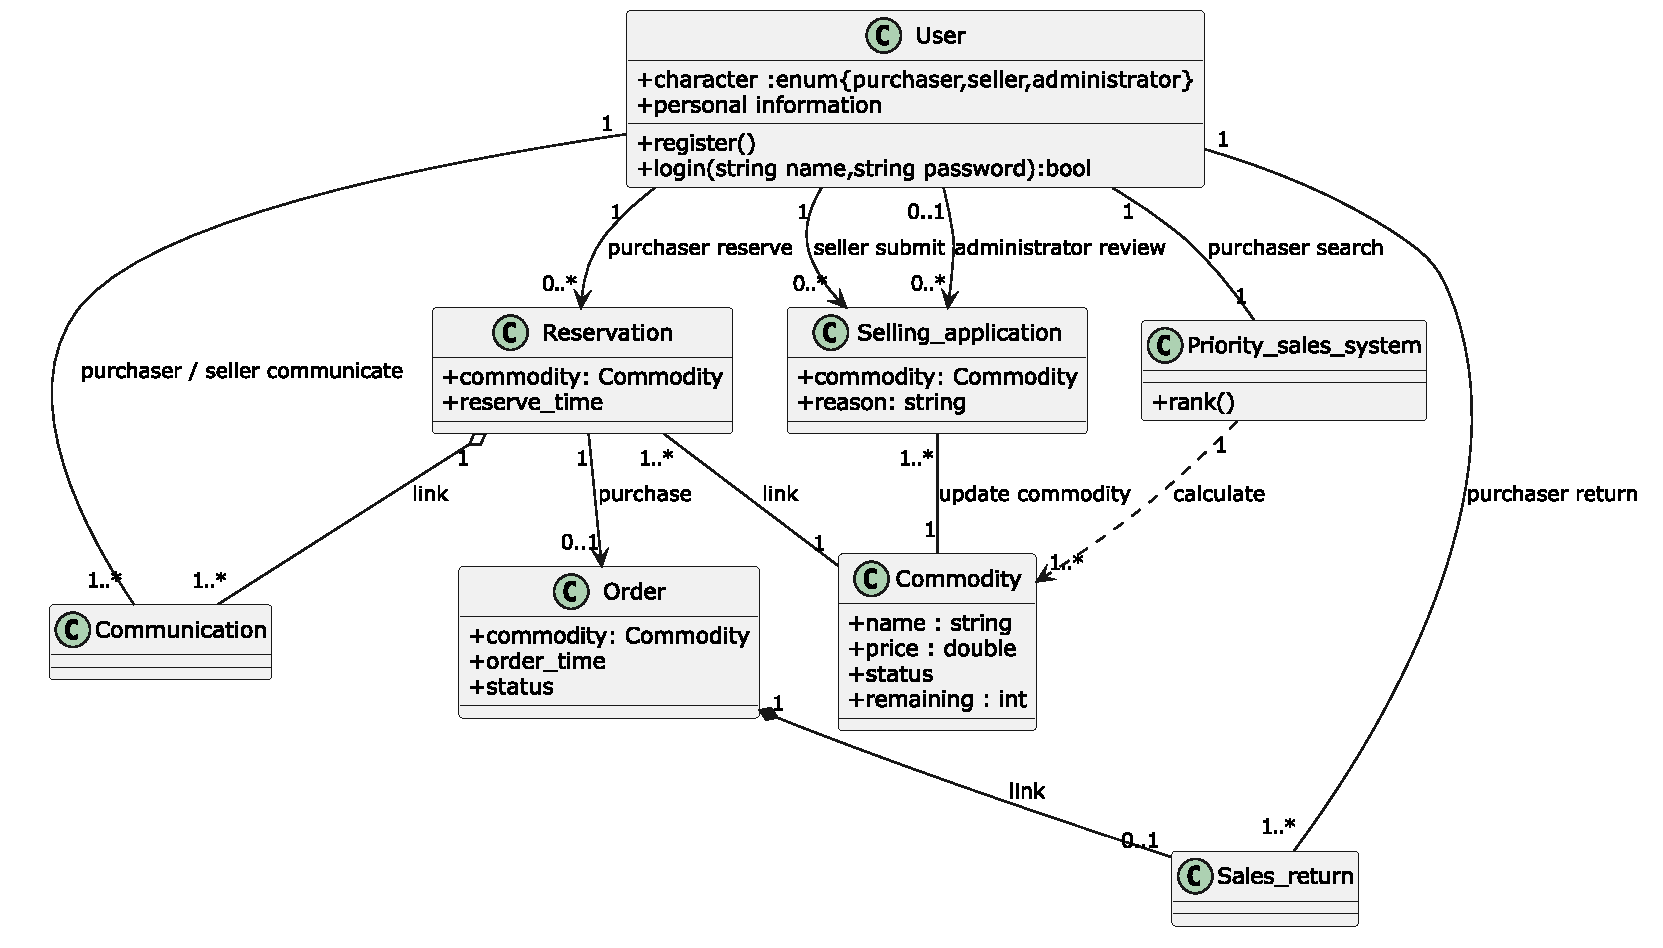
\includegraphics[width=\textwidth]{class-diagram.pdf}   % 实际路径 fig/class-diagram.pdf
    \caption{系统类图}
    \label{fig:class}
\end{figure}

如图~\ref{fig:class} 所示，系统主要包含以下类：
\begin{enumerate}
    \item User: 
        表示系统用户，包含属性：个人信息（personal information）（包括用户名，密码，其他隐私信息等等）与所代表的角色（character）\\
        对于身份（character），系统中有三种身份：管理员，买家，卖家。注意：虽然一个账号可以既是买家和卖家，
        但它们在系统中对应了权限和功能不一样，所以不能被视为同一个身份。\\
        对于功能，除了类中表明的注册（register）和登录（login）功能外，还包括其他用户相关操作，这些操作标注在了类间关系之中。\\
    \item Reservation:
        表示系统中的预约消息。当一个用户希望购买商品时，他必须提前预约这个商品。
    \item Commodity:
        表示系统中的商品。拥有属性：名称（name）\\
    \item Order:
        表示系统中的订单。拥有属性：订单号（order\_id）、商品（commodity）、用户（user）等\\
    \item Selling\_application:
        表示系统中的卖家申请\\
    \item Priority\_sales\_system:
        由于系统需要按照买家的一定偏好来推荐商品，所以需要这个优先级推荐系统。
        其中的方法（rank）用于对商品进行排序，返回一个排序后的商品列表。\\
    \item Sales\_return:
        表示系统中的退货申请\\
    \item Communication:
        表示买卖双方的信息交流\\
\end{enumerate}

\subsubsection{类间关系分析}
关联关系中以单向，双向为代表的一般的关联关系（类图中用link表示）比较常规，故不作说明。侧重于分析聚合，组合和依赖关系。\\
\begin{enumerate}
    \item Order 与 Sales\_return : 
        订单与退货申请之间的关系是组合关系。原因:根据本次实验中甲方的要求，
        一个退货申请必须依赖于一个订单，而一个订单未必需要有退货申请。即：退货申请必须依赖于订单存在。\\
    \item Communication 和 Reservation:
        买卖双方的交流和预约消息之间的关系是聚合关系。原因：一个预约消息可以包含多个交流信息，
        但交流信息不一定依赖于预约消息。\\
    \item Commodity 和 Priority\_sales\_system:
        商品和优先级推荐系统之间的关系是依赖关系。原因：优先级推荐系统需要对商品进行排序，
        但商品不依赖于优先级推荐系统的存在。\\
\end{enumerate}

\subsubsection{类图缺陷}

\begin{enumerate}
    \item User 实际上是抽象类，应派生出管理员、买家、卖家三个子类，并在各子类中分别列出其属性与方法；
    但这样会使类图过于庞杂、表达不清，因此图中改在类间关系上加以区分说明。
    \item 类图中未画出构造函数（如静态工厂的 create）、析构方法（如预约的取消）以及各类对应的 Service 类。
    原因是：一般的后端习惯按
    controller $\rightarrow$ application service $\rightarrow$ domain $\rightarrow$ repository/infrastructure
    分层，本图只描述领域（Domain）层，而领域类图应尽量与应用服务解耦。对象的创建与销毁虽由领域对象承载，
    但 create、delete 等操作的调用来自应用服务层，故不在领域类图中表达，以免与应用服务类图混淆。
\end{enumerate}

\section{UML 动态建模}

\subsection{用例图}
用例图描述参与者与系统功能之间的关系。

\begin{figure}[H]
    \centering
    % 图片源文件为 uml/instance.puml（PlantUML 导出）
    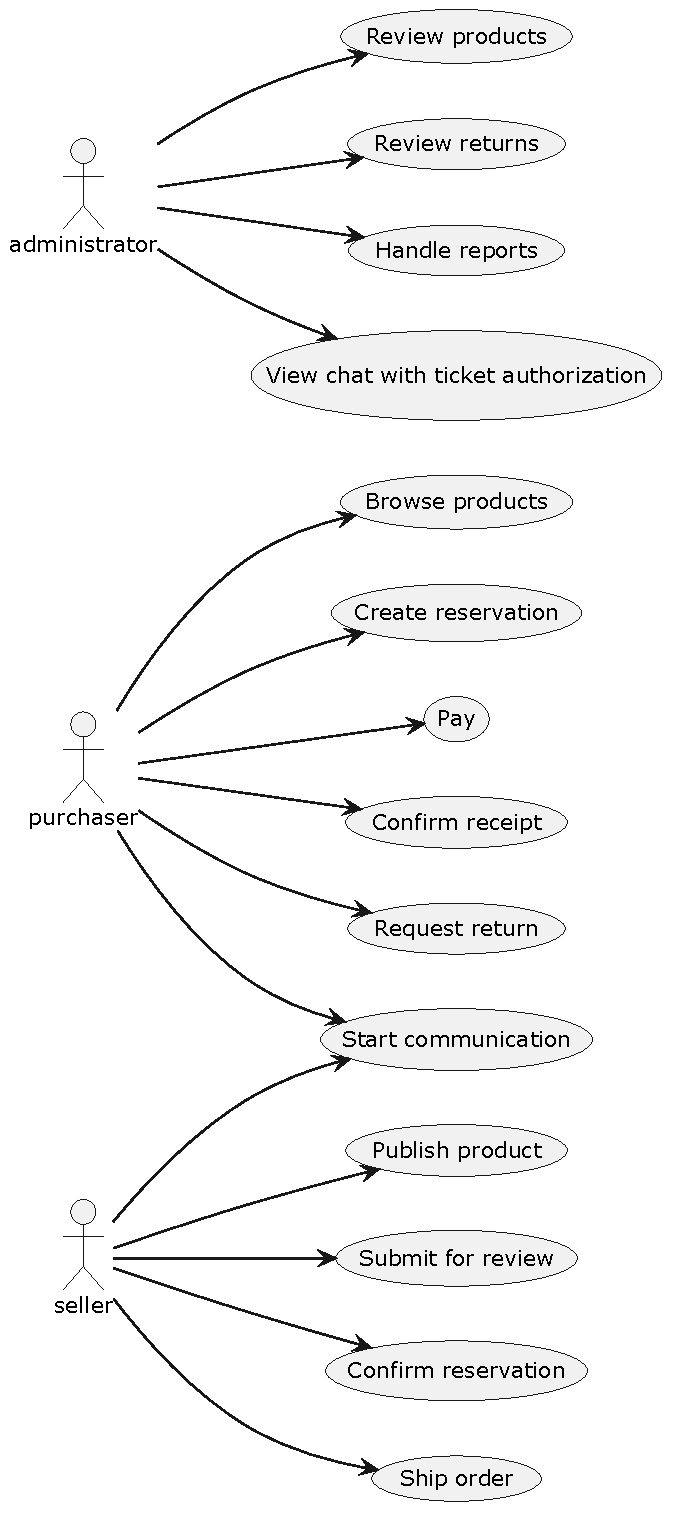
\includegraphics[width=0.5\textwidth]{use-case-diagram.pdf}
    \caption{系统用例图}
    \label{fig:usecase}
\end{figure}

如图~\ref{fig:usecase} 所示，系统共有三类参与者（实际为类图抽象类User的实际三个子类）：买家（purchaser）、卖家（seller）与管理员（administrator）。
\begin{enumerate}
    \item 买家可以浏览商品（Browse products）、发起预约（Create reservation）、付款（Pay）、
        确认收货（Confirm receipt）、发起退货（Request return）以及与卖家沟通（Start communication）；
    \item 卖家可以发布商品（Publish product）、提交审核（Submit for review）、确认预约（Confirm reservation）、
        发货（Ship order）以及与买家沟通（Start communication）；
    \item 管理员负责商品审核（Review products）、退货审核（Review returns）、处理举报（Handle reports），
        并可在有举报凭证时查看会话（View chat）。
\end{enumerate}
一个账号可以同时作为买家与卖家使用；管理员账号由系统预置，不参与买卖。

\subsection{时序图}
由于本次实验的关键部分在于从用户预约到完成交易部分，所以所列出的时序图重点解释这一核心点：

\begin{figure}[H]
    \centering
    % 图片源文件为 uml/sequence.puml（PlantUML 导出），
    % 这里用其矢量 PDF 版本插入，避免额外字体依赖
    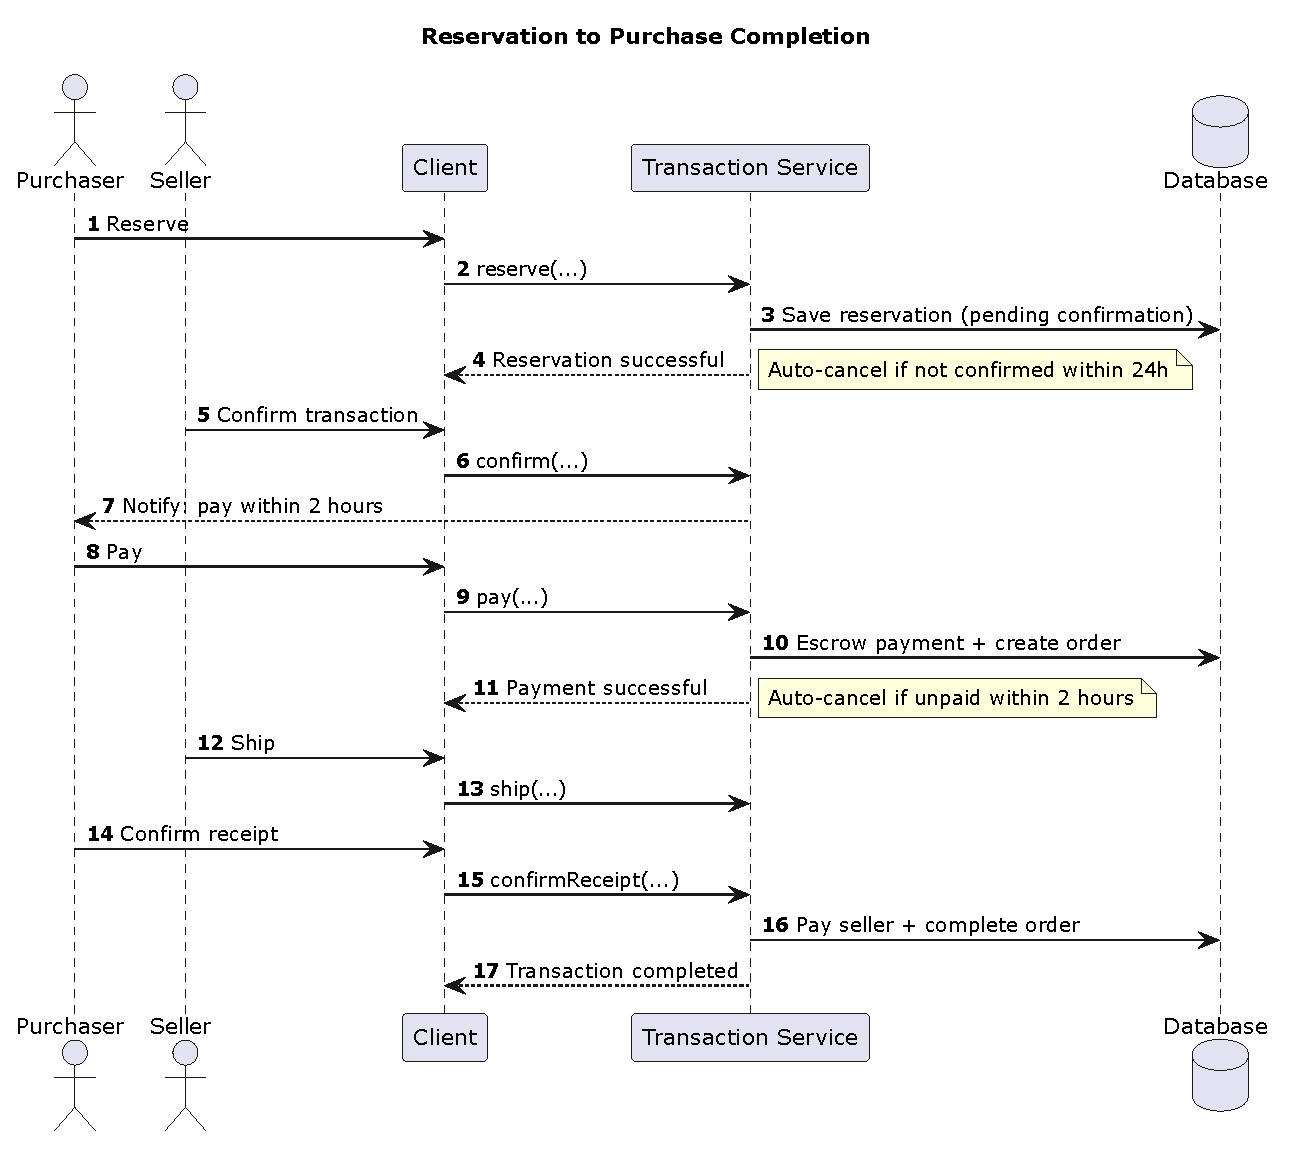
\includegraphics[width=\textwidth]{sequence-diagram.pdf}
    \caption{预约到交易完成的时序图}
    \label{fig:sequence}
\end{figure}

如图~\ref{fig:sequence} 所示，从预约到交易完成可分为以下几个阶段：
\begin{enumerate}
    \item 买家在客户端发起预约，客户端调用交易服务的 reserve 方法，交易服务向数据库写入
        “待卖家确认”的预约记录；卖家 24 小时内未确认的，系统自动取消预约并释放余量；
    \item 卖家在客户端确认交易，交易服务更新预约状态并通知买家在 2 小时内付款；
        逾期未付款的，预约自动取消并释放余量；
    \item 买家付款后，交易服务将货款存入平台托管并创建订单，此时卖家尚未收到货款；
    \item 卖家发货、买家确认收货后（且没有退货情况时），交易服务将托管货款打款给卖家，订单状态变更为已完成。
\end{enumerate}

\subsection{活动图}
活动图描述业务流程中活动的执行顺序与分支条件。

如图~\ref{fig:activity} 所示\\
\subsubsection{分支解释和额外说明}
\begin{enumerate}
    \item \textbf{预约是否有效?}预约的有效性来自于几个方面：
    除了活动图中标明的“商品存量大于0”以外，还要考虑商品是否违规等等因素；\\
    当确认有效时，减少库存为了保证数据一致性，应当是原子性的（atomic）。\\
    \item \textbf{卖家在 24 小时内确认 \&\& 买家在此期间未取消预约?}
    如图中所示，这两个条件应当是与（AND）的关系。\\
    取消预约后，减少的库存应即时返还给库存量。
    \item \textbf{卖家确认后生成订单,买家在 2 小时内付款?}
    订单有唯一的编号：order\_id，对于类图中order 的 order\_id 属性\\
    \item \textbf{卖家在 7 天内发货且买家在 7 天内收货?}卖家超期视为取消交易，买家超期视为完成交易\\
    \item \textbf{买家申请退货?}退货的成功不仅需要卖家确认，最后也需要管理员验收后，方可视为取消这笔订单，将平台托管的资金退还给买家。\\
\end{enumerate}



\begin{figure}[H]
    \centering
    % 图片源文件为 uml/activity.puml（PlantUML 导出）
    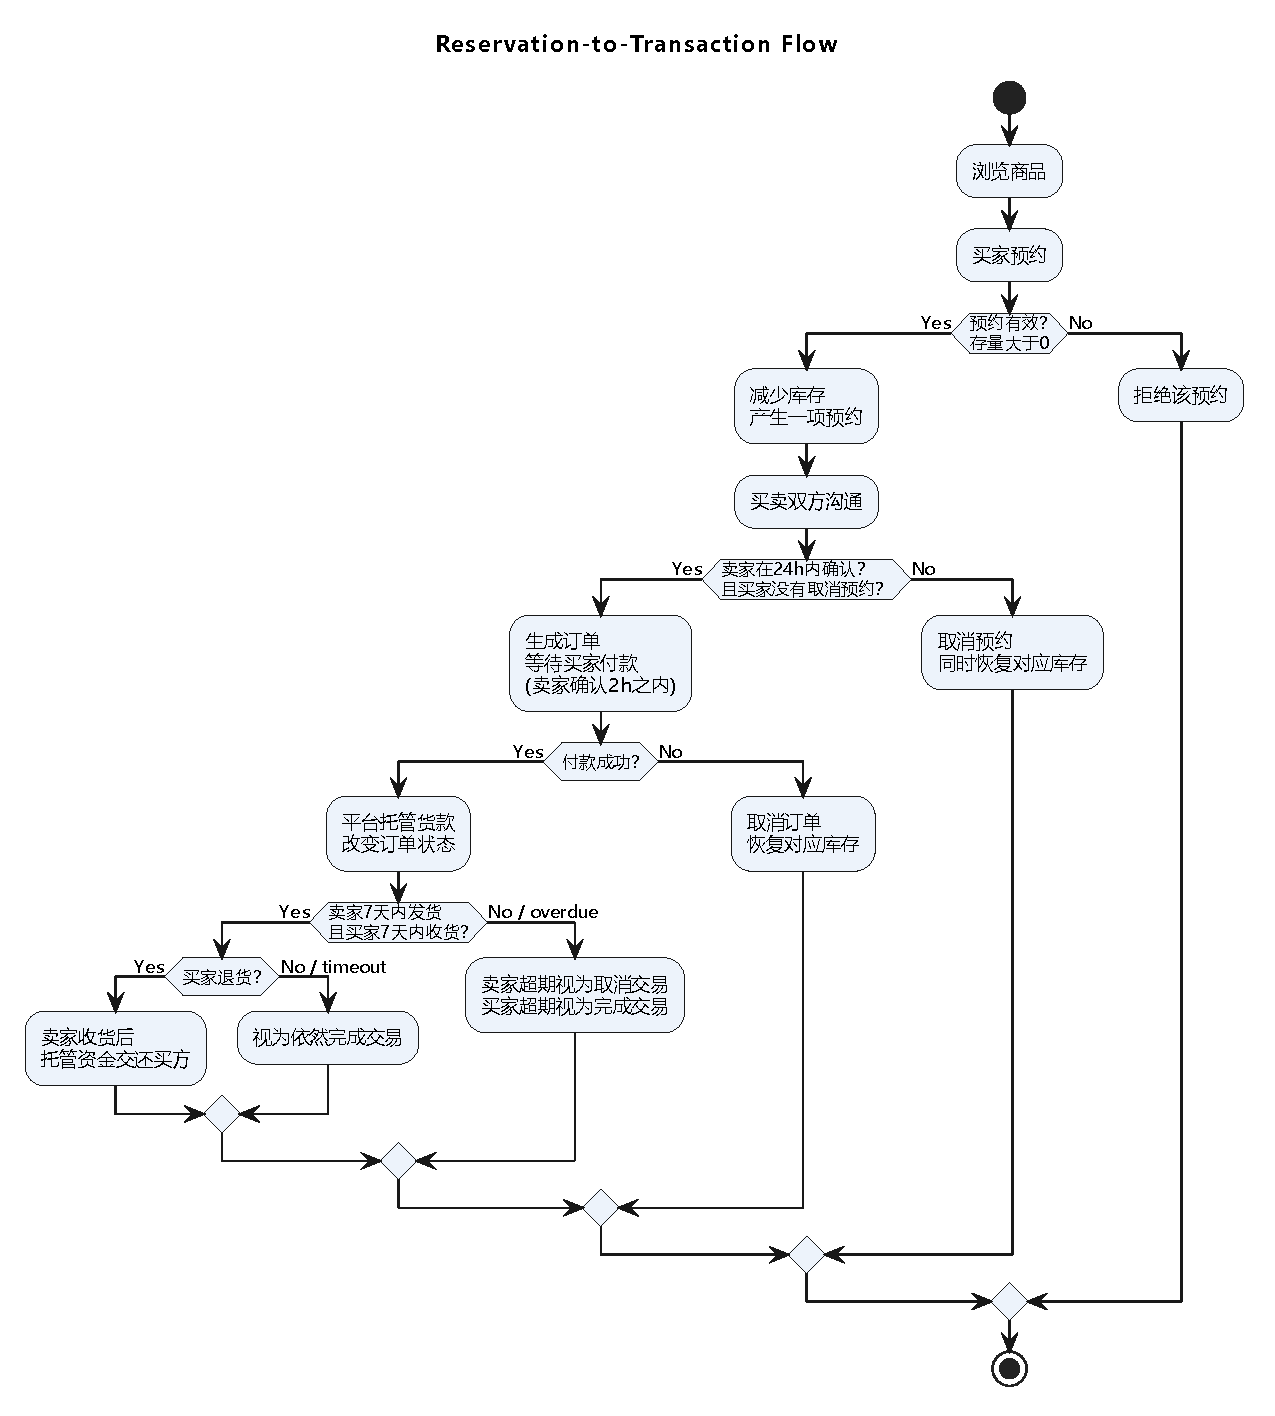
\includegraphics[width=0.95\textwidth]{activity-diagram.pdf}
    \caption{预约到交易完成的活动图}
    \label{fig:activity}
\end{figure}


\section{UI}

本节给出系统的三个核心界面原型：登录、商品浏览与订单管理。
界面仅用于展示信息结构与交互入口，具体业务逻辑由后端服务实现。

\subsection{登录界面}

\begin{figure}[H]
    \centering
    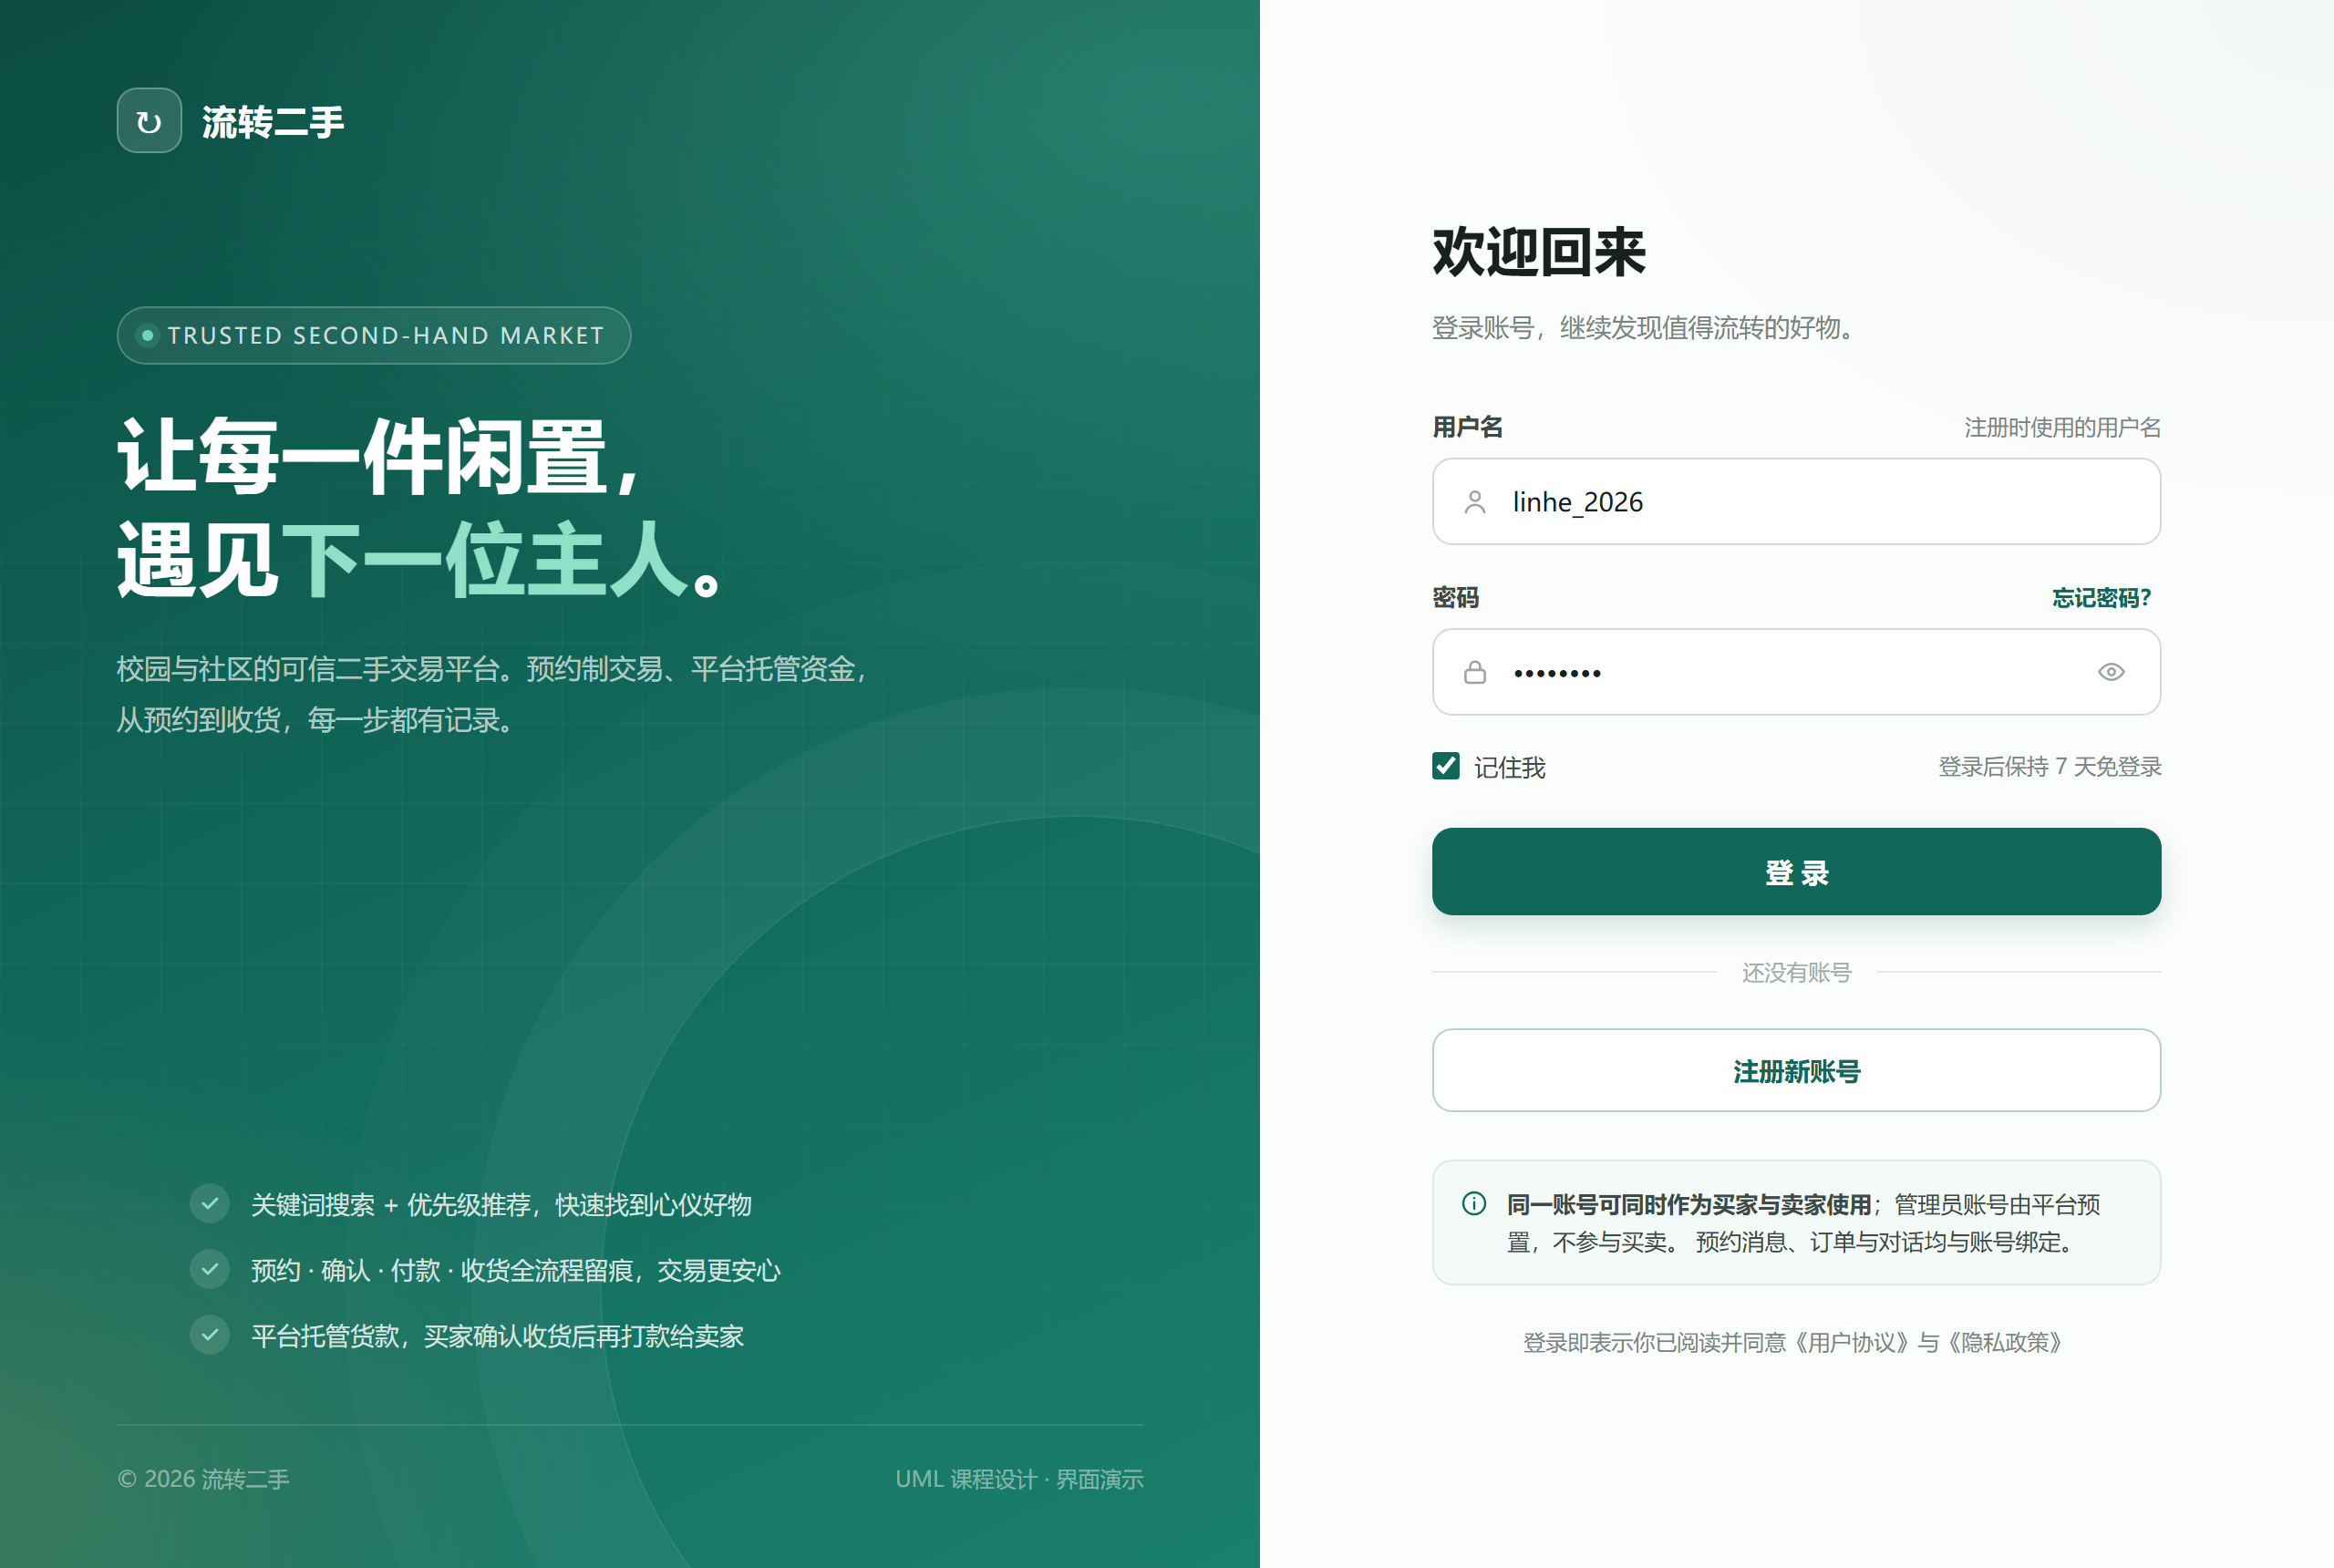
\includegraphics[width=\textwidth]{ui-login.png}
    \caption{登录界面}
    \label{fig:ui-login}
\end{figure}

如图~\ref{fig:ui-login} 所示，登录界面采用左右分栏结构：左侧展示平台定位与交易保障说明，
右侧为登录表单，包含用户名、密码、记住我与注册入口，分别对应类图中 User 类的 login(name, password)
与 register 操作。界面同时提示同一账号可同时作为买家与卖家使用，而管理员账号由平台预置。

\subsection{支持关键词的商品浏览界面}

\begin{figure}[H]
    \centering
    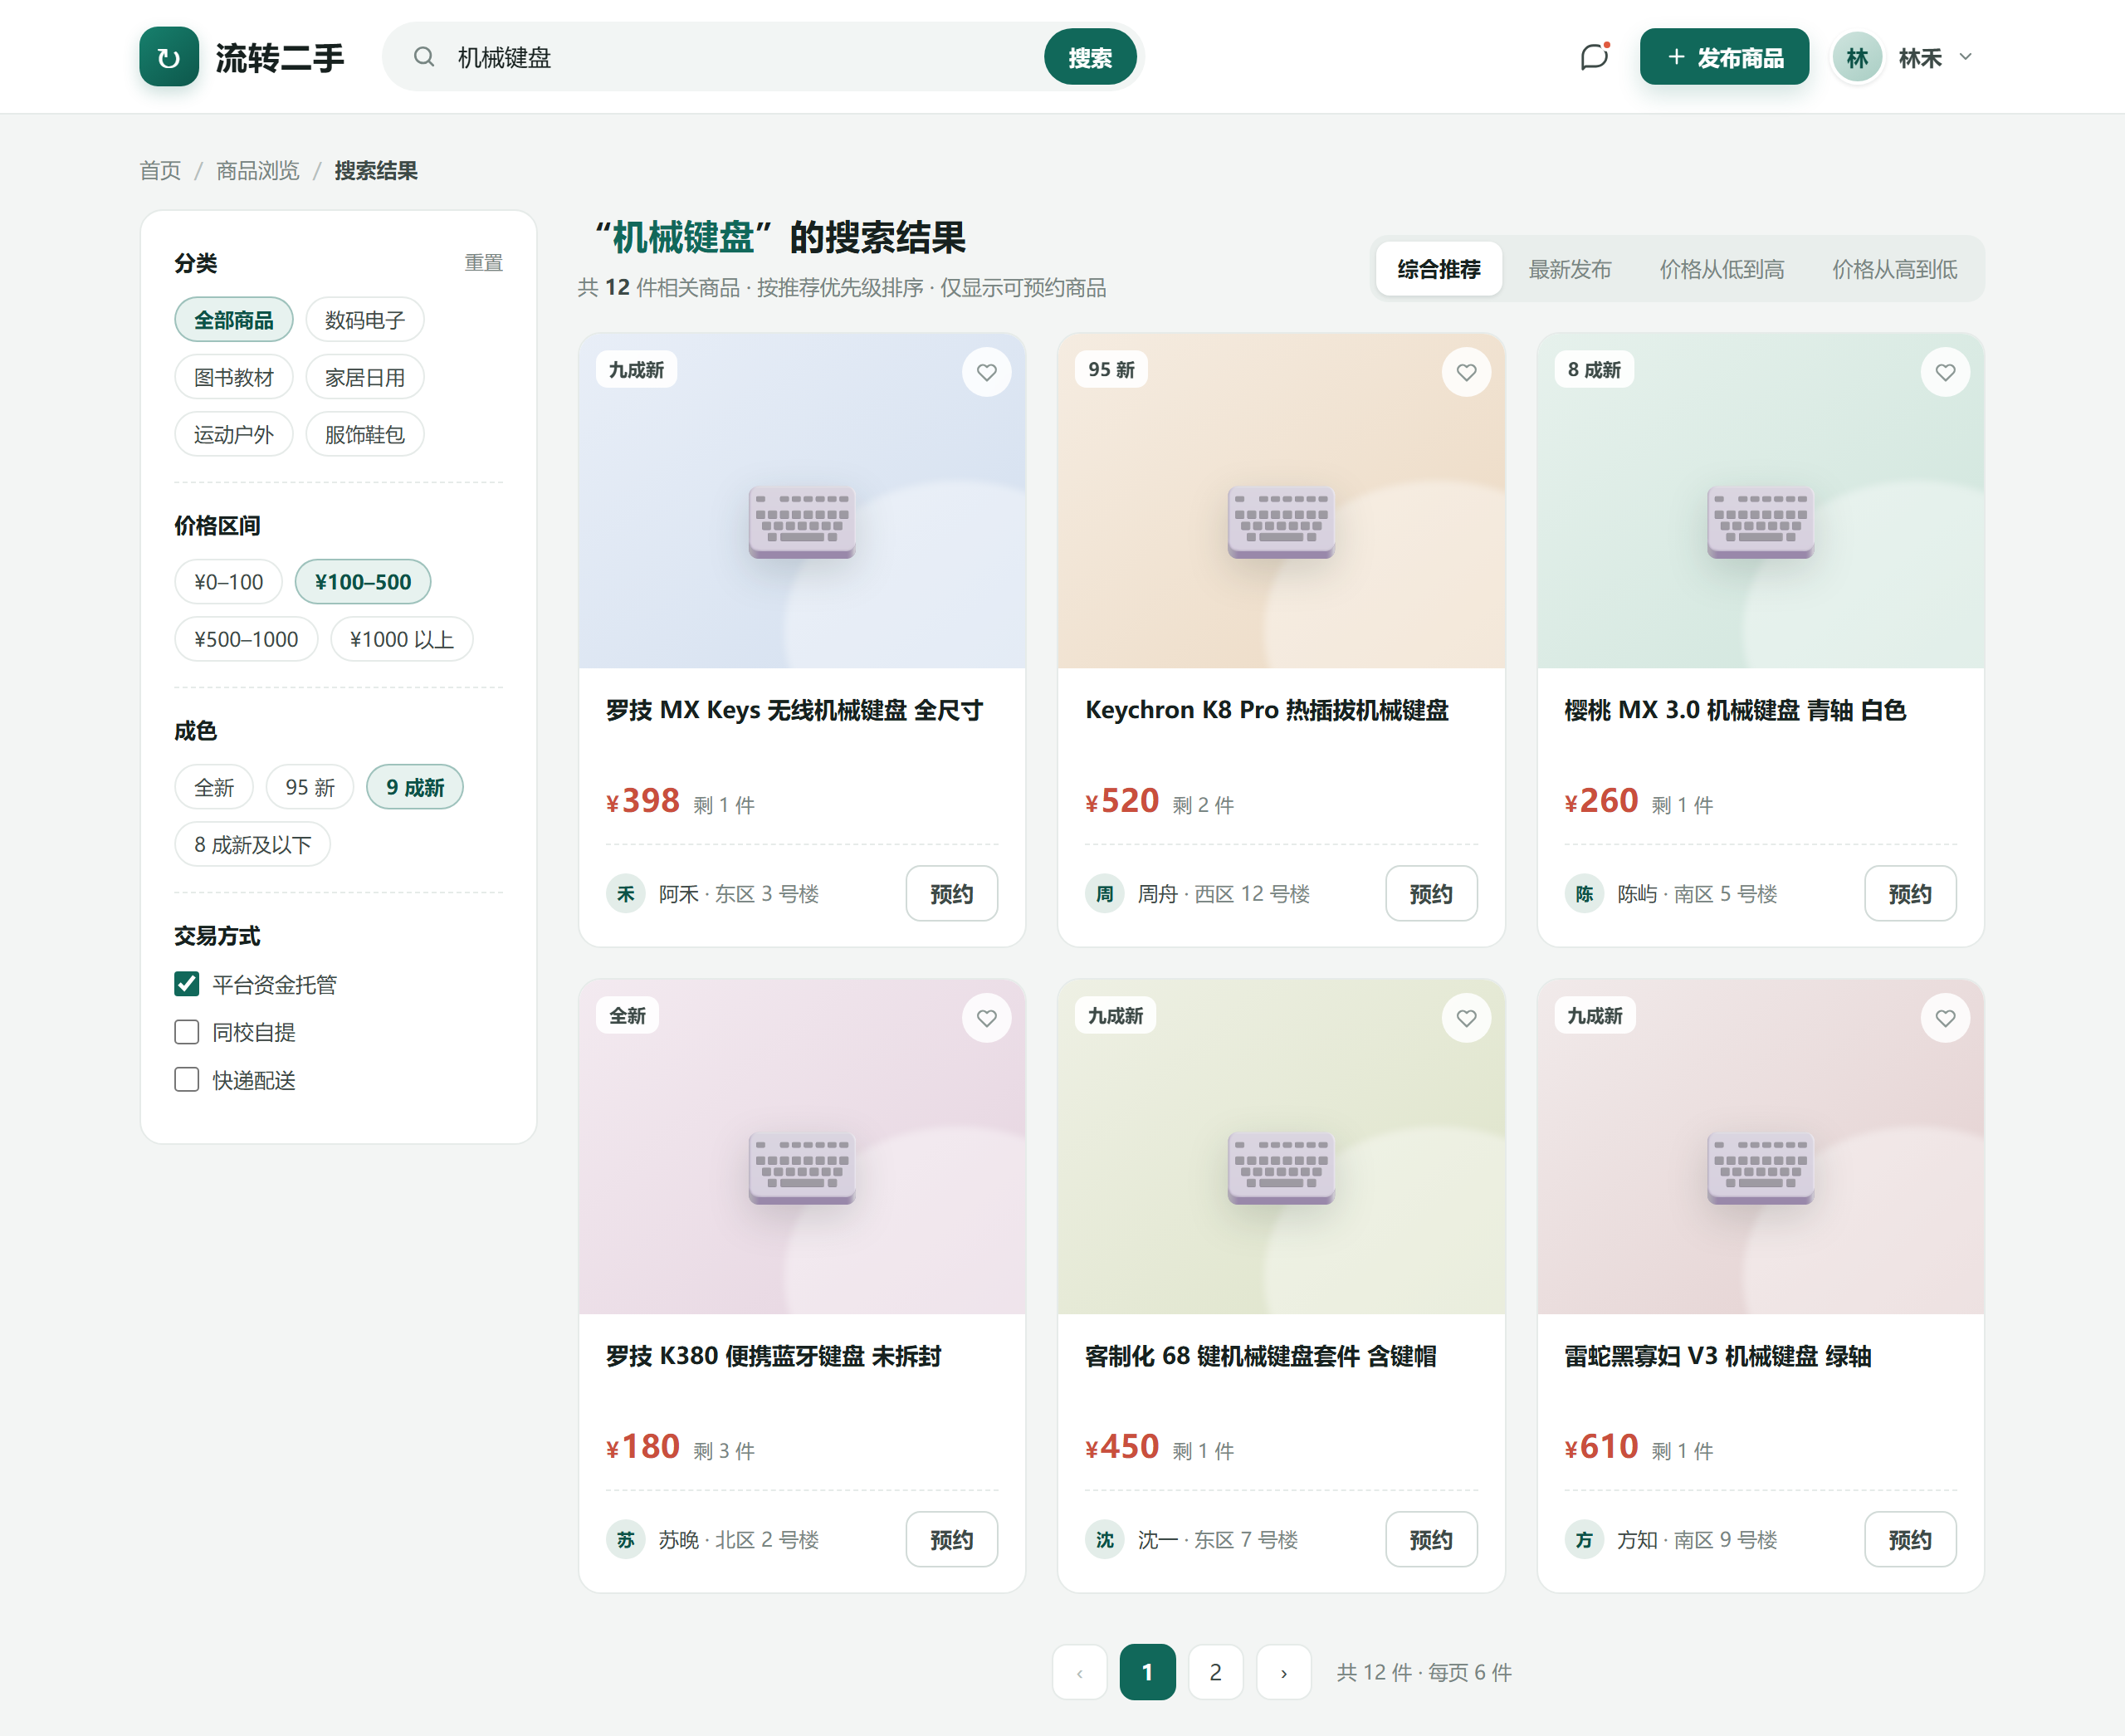
\includegraphics[width=\textwidth]{ui-browse.png}
    \caption{支持关键词搜索的商品浏览界面}
    \label{fig:ui-browse}
\end{figure}

如图~\ref{fig:ui-browse} 所示，界面顶部为关键词搜索框，左侧提供分类、价格区间、成色与交易方式四类筛选条件，
右侧以卡片形式展示商品名称、价格、剩余数量与卖家信息。“综合推荐”排序对应 Priority\_sales\_system 类的 rank 方法，
卡片上的“预约”按钮则对应买家发起预约（Create reservation）的用例。

\subsection{订单界面}

\begin{figure}[H]
    \centering
    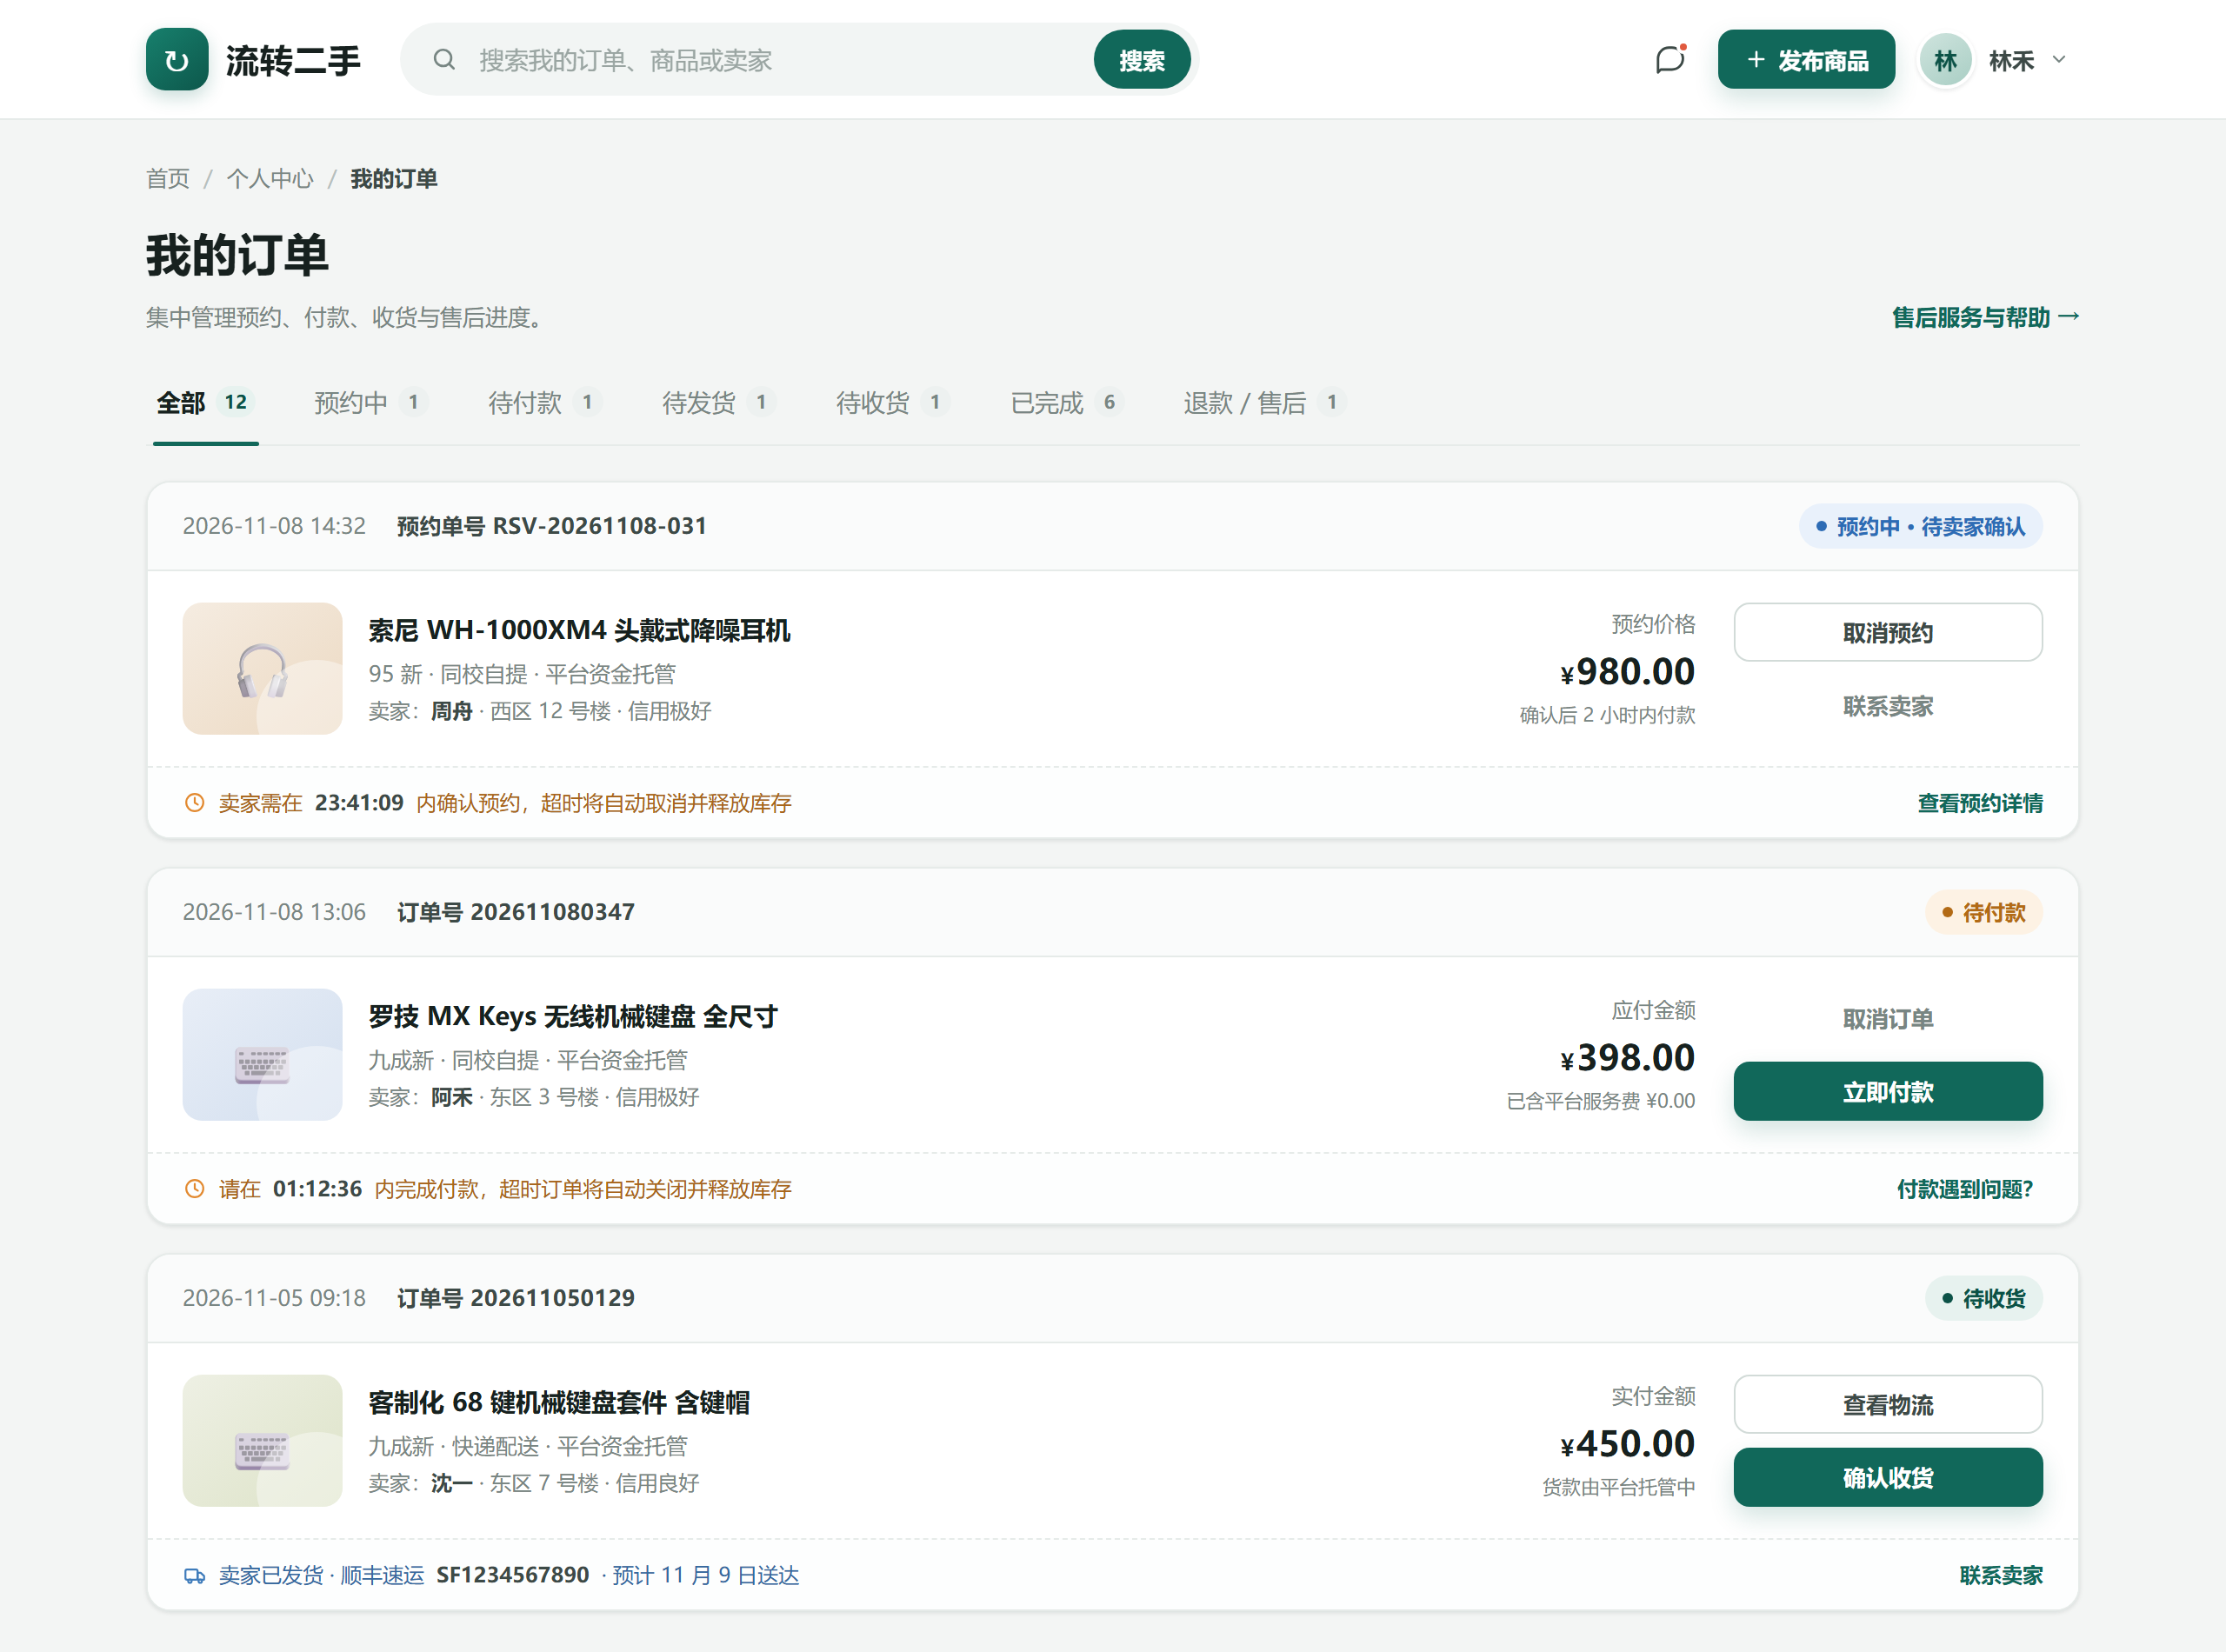
\includegraphics[width=\textwidth]{ui-orders.png}
    \caption{订单界面}
    \label{fig:ui-orders}
\end{figure}

如图~\ref{fig:ui-orders} 所示，订单界面按“预约中、待付款、待发货、待收货、已完成、退款/售后”对交易状态分组。
每张卡片展示预约单号或订单号、商品信息、金额与状态，并根据状态提供取消预约、立即付款、查看物流、
确认收货、申请退货等操作；卡片底部的倒计时对应时序图中预约 24 小时未确认、订单 2 小时未付款时自动取消并释放库存的规则。



\section{ai使用过程及思考}

\begin{enumerate}
    \item 首先，ai简化了很多繁杂的任务，
    比如给定.puml代码，在latex中插入uml图，使用几行prompt即可完成；抑或是中英文的转换翻译等等。\\
    \item 其次，ai可以润色口语化的表达并使其更严谨：(以3.0.2 类图缺陷为例)\\
        \fbox{%
            \begin{minipage}{0.8\textwidth}
                上述所有类，由于要创建实例，所以都默认应该有构造函数，比如说静态工厂模
式的 create 方法。有些类，比如说预约可以取消，所以也默认需要有一个析构方
法。除此以外，这些类由于要提供服务，所以最好还要有一个对应的 Service 类。
那为什么在类图中没有呢？
我觉得，主要是：应用服务类图和领域类图，表达的内容应该是不同的，所以形式
不同。
具体什么是应用服务，什么是领域？考虑到这个任务需要前后端分离，所以一般
的后端要如下地设计：
controller -> application service -> domain -> repository / infrastructure
对于上面这张类图中的类，实际上都是领域 Domain 层的对象，所以其表达的关
系主要就是领域的内容，需要尽量与 application service 的内容解耦。
而所谓 application service，包含的内容主要就是 create，delete（虽然这些方法
是应当加在领域对象中的，但对其的调用一定是来自于应用服务层）以及对应的
Service 
            \end{minipage}%
        } \\
        -> \\
        -> \\
        -> \\
        \fbox{%
            \begin{minipage}{0.8\textwidth}
                类图中未画出构造函数（如静态工厂的 create）、析构方法（如预约的取消）以及各类对应的 Service 类。
    原因是：一般的后端习惯按
    controller $\rightarrow$ application service $\rightarrow$ domain $\rightarrow$ repository/infrastructure
    分层，本图只描述领域（Domain）层，而领域类图应尽量与应用服务解耦。对象的创建与销毁虽由领域对象承载，
    但 create、delete 等操作的调用来自应用服务层，故不在领域类图中表达，以免与应用服务类图混淆。
            \end{minipage}%
        }

\end{enumerate}




\end{document}
